\documentclass[conference]{IEEEtran}
\usepackage{graphicx}
\usepackage{amsmath,amssymb}
\usepackage{booktabs}
\usepackage{tabularx}
\usepackage{cite}
\usepackage{xcolor}
\usepackage{url}

% Anything in \tbd{...} must be filled in or checked before submission.
\newcommand{\tbd}[1]{\textcolor{red}{#1}}

\begin{document}

\title{Camera-Only Metric 3D Object Boxes from Monocular Video:\\Initial Results}

\author{\IEEEauthorblockN{\tbd{Name One (student no.), Name Two (student no.), Name Three (student no.)}}
\IEEEauthorblockA{AER1515 Perception for Robotics, University of Toronto}}

\maketitle

\begin{abstract}
We study how well a robot can find everyday objects in 3D using only a moving colour camera. Boxer, a recent open-world method from Meta Reality Labs, turns 2D object detections into metric 3D boxes and outperforms the prior lifting methods it is compared with, but its accuracy falls by more than half without a depth sensor. We reimplemented Boxer's unreleased evaluation and reproduced its published results on the CA-1M dataset to within 0.01--0.04 mAP. We then replaced the depth sensor with depth predicted from each single image by Depth Anything~3. Although this depth is within 9\% of the sensor on average, it recovers almost none of the lost accuracy: 0.101 mAP, against 0.100 without depth and 0.216 with the sensor. We show that 3D overlap scoring is far stricter than 2D scoring, so depth errors of a few percent move boxes further than many objects are wide. These results motivate the next stages of the project: multi-view depth that is metrically consistent across frames, and a multi-view refinement of each box.
\end{abstract}

\section{Problem and Applications}
We want the \emph{metric} 3D bounding box of every object in a room, meaning its position, size and heading in metres, from an ordinary video with no depth sensor. Robots and augmented-reality (AR) devices need this to know which objects are nearby and how large they are. It enables object maps for navigation and grasping, queries such as ``where is the mug?'', and cheaper hardware without LiDAR.

Our starting point is Boxer~\cite{boxer}, accepted at ECCV 2026. It was developed at Meta Reality Labs and is demonstrated on recordings from Project Aria AR glasses as well as on iPad and RGB-D datasets. Boxer is given 2D boxes from an image detector and \emph{lifts} each one to a 3D box. In its own benchmarks it outperforms the prior lifting method CuTR~\cite{ca1m} with every input it was tested on. It relies heavily on depth, however: on CA-1M~\cite{ca1m}, with detector boxes, its accuracy drops from 0.204 to 0.081 mAP, the score defined in Sec.~\ref{sec:metric}, when the depth input is removed. It also assumes that the camera pose and the direction of gravity are known. Our research question is how much of this gap between RGB-only and RGB-D input a camera-only pipeline can close, and which component closes it.

\section{Relationship to Course}
The project combines 3D object detection by lifting 2D boxes to 3D, deep monocular and multi-view depth estimation, multi-view geometry with camera poses, triangulation and SLAM, nonlinear least squares with robust losses for our planned box refinement, and uncertainty modelling, since Boxer's predicted uncertainty serves as a measurement weight. Together these make up a robotic-perception problem: building a metric object map from a single onboard camera.

\section{Solution Method}
\subsection{Baseline: how Boxer works}
Fig.~\ref{fig:pipeline} shows Boxer's pipeline for each video frame. Its inputs are the colour image; the camera \emph{pose}, which gives the camera's position $x,y,z$ and its rotation as roll, pitch and yaw, together with the direction of gravity; and an optional depth image giving the distance to the scene at each pixel. All boxes and poses are expressed in one fixed room coordinate frame whose $z$ axis points up, against gravity.
First, a \emph{2D detector}, OWLv2~\cite{owlv2}, is prompted with about 1{,}200 object names and returns 2D boxes with confidence scores.
Second, \emph{BoxerNet} resizes the image to $960\times960$ pixels and cuts it into a $60\times60$ grid of $16\times16$-pixel patches. Each patch is described by its appearance, using DINOv3 features~\cite{dinov3}, by the direction of its viewing ray, computed from the pose and the camera intrinsics, and by its mean depth when depth is available. Each 2D box attends to these patches and predicts one 3D box: a centre, a width, length and height, and a yaw angle about the vertical axis, so boxes are always upright. It also predicts an uncertainty that is converted into a confidence.
Third, \emph{fusion} merges boxes of the same object from different frames whenever their 3D overlap exceeds 0.3, using confidence-weighted averaging, which yields one box per object for the whole room.

\begin{figure*}[t]
\centering
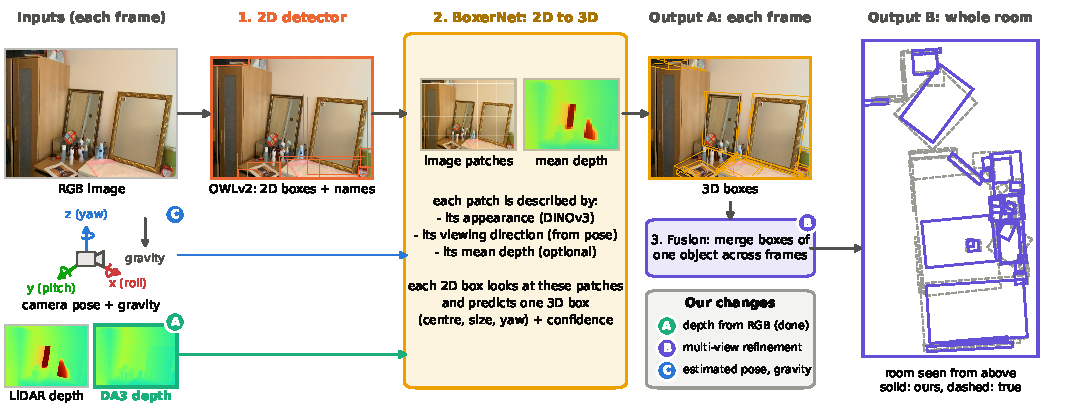
\includegraphics[width=\textwidth]{fig_pipeline.pdf}
\caption{Boxer's pipeline on a real CA-1M frame. Stage~1 draws 2D boxes, stage~2 lifts each to a 3D box and stage~3 fuses boxes across frames into a room map, shown from above with predictions solid and true boxes dashed. In stage~2 the patch grid is drawn four times coarser than BoxerNet's real $60\times60$ grid so that it remains visible; the depth map is shown at the true patch resolution. Badges mark the parts we replace: A, depth predicted from the image (done); B, a multi-view refinement in place of fusion; C, estimated pose and gravity.}
\label{fig:pipeline}
\end{figure*}

\subsection{Our approach}
We keep the detector and the BoxerNet weights fixed and replace, in three stages, the parts that require extra sensors.

\textbf{Stage A: predicted depth.} Depth predicted from the camera images is given to Boxer in place of LiDAR and sampled exactly like the sensor depth. We test three representative sources: DA3METRIC-LARGE~\cite{da3}, which predicts metric depth from a single image and is complete; DA3-Nested-Giant~\cite{da3}, which uses many frames and can take the known camera poses as input, with MapAnything~\cite{mapanything} as an alternative; and one single-image metric model from a different family, MoGe~\cite{moge} or UniDepth~\cite{unidepth}. VGGT~\cite{vggt} is optional because of its memory cost. Each source is scored both by its depth error against LiDAR and by the mAP it produces.

\textbf{Stage B: multi-view box refinement.} We replace fusion's averaging with a per-object optimization over all frames $f$ in which the object is seen:
\begin{equation}
\begin{split}
B^* = \arg\min_B\; &\sum_f w_f\,\rho\big(\lVert \pi(B,T_f)-b_f\rVert^2\big)\\
&+ \lambda \sum_p w_p\,\rho\big(d(p,B)^2\big),
\end{split}
\label{eq:refine}
\end{equation}
where $\pi(B,T_f)$ projects box $B$ into frame $f$ with pose $T_f$, $b_f$ is the detected 2D box, $d(p,B)$ is the distance from a predicted 3D point $p$ to the box, $\rho$ is the Huber loss and the weights $w$ come from BoxerNet's uncertainty. It is solved with Levenberg--Marquardt starting from the fused box, and each term is ablated.

\textbf{Stage C: fully camera-only.} Poses are estimated with MASt3R-SLAM~\cite{mast3rslam} or VGGT~\cite{vggt} and gravity with GeoCalib~\cite{geocalib}, and the loss relative to the device's ARKit poses is reported.

\textbf{Optional objective: other 2D detectors.} Only if time allows, we will replace OWLv2 with newer open-world detectors such as YOLO-World~\cite{yoloworld}, Grounding DINO~\cite{groundingdino} and SAM~3~\cite{sam3}, since the detector limits recall before depth matters (Sec.~\ref{sec:analysis}).

\textbf{Compute.} All experiments run on an RTX~5080 GPU with 16\,GB of memory, owned by \tbd{team member name}. A full evaluation of 6{,}157 frames takes 5--8\,min for Boxer and about 5\,min for DA3 depth.

\section{Dataset and Evaluation}
\subsection{CA-1M}
CA-1M~\cite{ca1m} contains iPad videos of indoor rooms. Its 3D boxes were annotated on a separate high-accuracy laser scan, so the ground truth is independent of the iPad's own depth and poses. Each frame also comes with iPad LiDAR depth, which serves as our upper bound, and ARKit poses. We use Boxer's ten validation videos, with 6{,}157 frames and 887 distinct objects. As in~\cite{boxer}, floors, walls and objects larger than 3\,m are removed, and box sides shorter than 5\,cm are expanded to 5\,cm. ScanNet++~\cite{scannetpp} remains an optional second dataset for checking generalization.

\subsection{Metric}
\label{sec:metric}
The 3D \emph{intersection over union} (IoU) of a predicted and a true box is their shared volume divided by their combined volume; it is 1 for identical boxes and 0 for boxes that do not touch. A prediction is correct if its IoU with a not-yet-matched true box exceeds a threshold. Ranking predictions by confidence gives \emph{precision}, the fraction of predictions that are correct, and \emph{recall}, the fraction of true objects that are found. \emph{Average precision} (AP) is the area under the precision--recall curve, so missed objects cap recall below 1 and directly lower AP. Following~\cite{boxer,omni3d}, mAP is the mean AP over IoU thresholds from 0.05 to 0.50 in steps of 0.05. Labels are ignored, so a correct box with the wrong name still counts. \emph{Per-frame} scores compare the boxes in each frame with the objects visible in that frame; \emph{per-scene} scores compare the fused room map with all objects seen.

Boxer's evaluation code is not released, so we reimplemented it. Where the paper is silent, we use COCO-style 101-point AP with detections pooled over all frames, and evaluate every frame. IoU is computed with Boxer's own function for upright boxes. Most true boxes are upright, but 2.6\% are tilted by more than 20$^\circ$, for example mirrors leaning against a wall, and these are scored as if upright.

\subsection{Why 3D IoU is a harsh metric}
\label{sec:iou}
Consider a cube of side $L$ and a prediction of the correct size shifted by $\epsilon L$ along every axis. In $d$ dimensions the overlap is $L^d(1-\epsilon)^d$ and the union is $2L^d-L^d(1-\epsilon)^d$, so
\begin{equation}
\mathrm{IoU}_d=\frac{(1-\epsilon)^d}{2-(1-\epsilon)^d}.
\end{equation}
A 10\% shift gives an IoU of 0.82 in 1D, 0.68 in 2D and only 0.57 in 3D. Solving for the largest shift that still passes IoU\,$\ge$\,0.5 gives 33\% in 1D but only 12.6\% in 3D, so the centre of a 10\,cm object must be within about 1.3\,cm on every axis. Size errors compound in the same way: a box 10\% too large in every direction scores 0.75 in 3D but 0.91 in 1D. Together with the many small objects and the missed detections described in Sec.~\ref{sec:analysis}, this explains why absolute mAP values are low even with measured depth. Class confusion plays no part, because labels are ignored.

\section{Initial Results}
\label{sec:results}
\subsection{Reproducing Boxer}
Table~\ref{tab:repro} compares our evaluation of the released Boxer with its published numbers. Per-frame scores lie within 0.01--0.04 of the paper and preserve its ranking, which validates our evaluation code. Per-scene scores agree less well. Enabling the paper's final duplicate-removal step, 3D non-maximum suppression at IoU 0.6, which is disabled by default in the released code, changed nothing, because fusion has already merged every pair of boxes that overlap by more than 0.3. The remaining per-scene difference is unexplained, so per-frame mAP is our primary metric.

\begin{table}[t]
\caption{Reproduction of Boxer on CA-1M (mAP). ``Found'' is per-frame recall at IoU\,0.05, the share of true objects that receive any box.}
\label{tab:repro}
\centering
\setlength{\tabcolsep}{3.5pt}
\begin{tabular}{llccccc}
\toprule
& & \multicolumn{2}{c}{Per-frame} & \multicolumn{2}{c}{Per-scene} & \\
2D boxes & Depth & paper & ours & paper & ours & Found \\
\midrule
OWLv2 & LiDAR & 0.204 & 0.216 & 0.204 & 0.288 & 43.6\% \\
OWLv2 & none  & 0.081 & 0.100 & 0.081 & 0.095 & 33.4\% \\
true  & LiDAR & 0.412 & 0.450 & 0.434 & 0.404 & 81.5\% \\
true  & none  & 0.126 & 0.157 & 0.089 & 0.116 & 54.0\% \\
\bottomrule
\end{tabular}
\end{table}

\subsection{Depth predicted from a single image}
Table~\ref{tab:depth} shows Boxer with OWLv2 boxes and three depth inputs. DA3METRIC-LARGE converts its output to metres using the camera's focal length, as its authors specify. Against LiDAR its depth is good by the usual depth measures: a mean relative error of 8.7\%, or 16\,cm; a global scale of 0.97, meaning about 3\% too close; and 91\% of pixels within 25\%. Yet it closes only about 1\% of the per-frame gap and 7\% of the per-scene gap. In Fig.~\ref{fig:results}a the DA3 curve lies on the no-depth curve at every threshold, and Fig.~\ref{fig:results}b shows no gain for any object size.

\begin{table}[t]
\caption{Depth source with OWLv2 2D boxes. Depth error is measured against iPad LiDAR. Gap closed $=(\text{mAP}-\text{mAP}_\text{none})/(\text{mAP}_\text{LiDAR}-\text{mAP}_\text{none})$, per frame.}
\label{tab:depth}
\centering
\setlength{\tabcolsep}{3pt}
\begin{tabular}{lcccccc}
\toprule
Depth & rel.\ err & scale & mAP & mAP & mAP & gap \\
 & & & frame & scene & small & closed \\
\midrule
none            & --    & --   & 0.100 & 0.095 & 0.027 & 0\% \\
DA3METRIC (RGB) & 8.7\% & 0.97 & 0.101 & 0.108 & 0.031 & 1\% \\
iPad LiDAR      & ref.  & ref. & 0.216 & 0.288 & 0.096 & 100\% \\
\bottomrule
\end{tabular}
\end{table}

\begin{figure}[t]
\centering
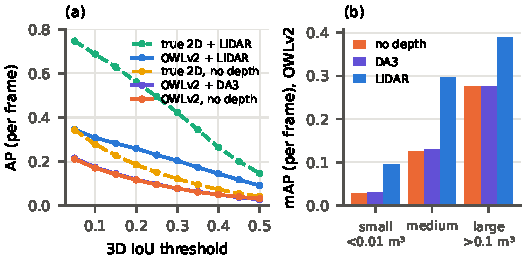
\includegraphics[width=\columnwidth]{fig_results.pdf}
\caption{(a) Per-frame AP versus the IoU required to count as correct. (b) Per-frame mAP by object volume with OWLv2 boxes. Small objects, the largest group with 28.8k of 65.2k per-frame instances, almost always fail without accurate depth.}
\label{fig:results}
\end{figure}

\begin{figure*}[t]
\centering
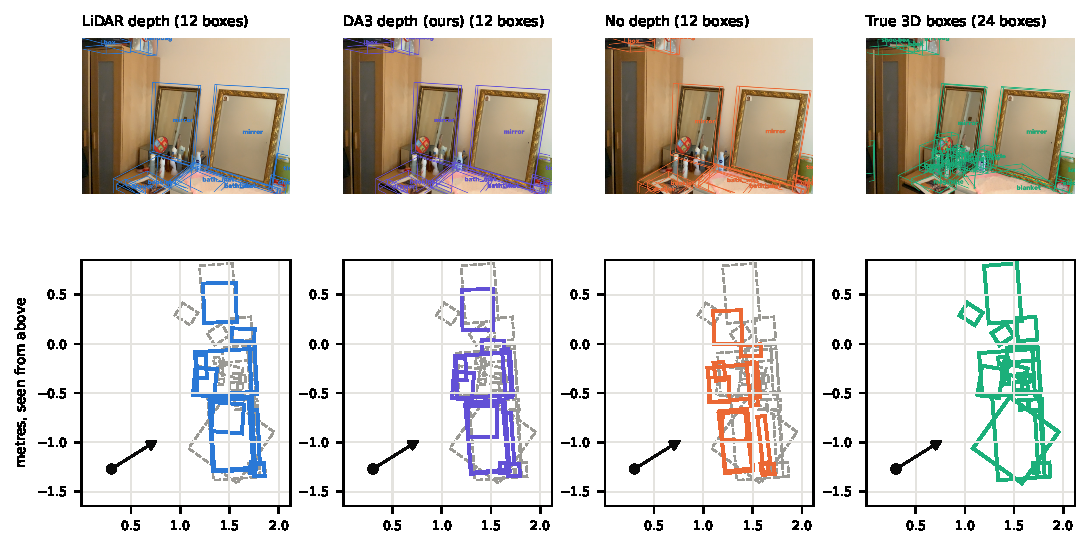
\includegraphics[width=0.92\textwidth]{fig_qualitative.pdf}
\caption{One CA-1M frame. Top: 3D boxes drawn on the image for each depth input, and the true boxes; object names are shown for illustration and are not scored. Bottom: the same boxes seen from above, with true boxes dashed in grey and the camera shown as a dot and arrow. From the camera, all predictions look alike, because a box that is too far away and too large projects to the same outline. From above, the boxes from DA3 and from no depth are displaced from the true boxes, while the LiDAR boxes match them more closely. Boxer kept 12 boxes in this frame; there are 24 true objects.}
\label{fig:qual}
\end{figure*}

\subsection{Analysis}
\label{sec:analysis}
\textbf{Why good depth does not help.} Sec.~\ref{sec:iou} shows that 3D IoU tolerates only centimetre errors for small objects. A depth error of 3--5\% at a typical range of 2--3\,m moves a box by 10--15\,cm, more than the width of most small objects. Without a depth input, BoxerNet already estimates distance from the image itself, and depth with errors of this size evidently adds little to that estimate. Fig.~\ref{fig:qual} shows the effect: boxes from DA3 and from no depth look the same from the camera but sit in the wrong place when seen from above. The DA3 error is mostly a consistent scale offset, about 5\% too close across the frame in Fig.~\ref{fig:qual}, and the offset varies between videos from 0.87 to 1.01. This is the key reason for our next step: depth that is metrically consistent across frames, from multi-view and pose-conditioned models that can fix the scale using the known camera motion. LiDAR is not perfect either, since it measures the reflection in mirrors, where DA3 is more accurate.

\textbf{Limited views.} A single frame shows only the front surfaces of an object, so neither the image nor any depth map reveals how far the object extends backwards. Its depth extent must be inferred, which mainly affects size and therefore IoU. Viewing the object from several directions removes this ambiguity, which is a further motivation for multi-view refinement.

\textbf{Missed objects.} Recall is limited before depth matters. With perfect 2D boxes, Boxer gives some box to 81.5\% of objects; with OWLv2 boxes, only 43.6\%, even with LiDAR. The detector therefore misses about 38\% of objects outright, mostly small ones, and no depth model can recover them. OWLv2 also removes duplicates only among boxes with the same name, so ``drawer'' and ``dresser'' boxes on one object both survive and count as false positives in class-agnostic scoring. Without depth, fusion also fails to merge boxes of the same object, leaving 1{,}225 room boxes for 887 objects when perfect 2D boxes are used.

\textbf{What a low mAP means in practice.} The boxes fit their objects well in the image, as Fig.~\ref{fig:qual} shows; the errors lie mainly in distance and size. A low-compute monocular manipulator that re-observes an object as it approaches could therefore already use such boxes, because a fixed relative depth error shrinks in absolute terms as the range decreases, and depth estimated from camera motion is expected to reduce it further.

\section{Updated Timeline}
\begin{table}[h]
\caption{Project timeline. Deliverables are in bold; each is due on the last date of its row.}
\label{tab:timeline}
\centering
\renewcommand{\arraystretch}{1.15}
\setlength{\tabcolsep}{3pt}
\begin{tabularx}{\columnwidth}{@{}l>{\raggedright\arraybackslash}Xl@{}}
\toprule
Dates & Work & Status \\
\midrule
\tbd{Sep.}--Oct.~9 & Literature review and method selection; \textbf{proposal} & Done \\
Oct.~10--Nov.~13 & Set-up; evaluation reimplemented and Boxer reproduced; DA3METRIC tested; \textbf{initial results} & Done \\
Nov.~14--20      & DA3-Nested with known poses; MoGe or UniDepth; depth error against LiDAR & Next \\
Nov.~21--27      & First version of the multi-view refinement; \textbf{demonstration video} & Planned \\
Nov.~28--Dec.~4  & Refinement ablations; camera-only run with estimated poses and gravity & Planned \\
Dec.~5--11       & Analysis by object size and component; optional detector study; \textbf{final report} & Planned \\
\bottomrule
\end{tabularx}
\end{table}

\begin{thebibliography}{99}
\bibitem{boxer} D.~DeTone \emph{et al.}, ``Boxer: Robust lifting of open-world 2D bounding boxes to 3D,'' in \emph{Proc. Eur. Conf. Comput. Vis. (ECCV)}, 2026, arXiv:2604.05212.
\bibitem{ca1m} J.~Lazarow, D.~Griffiths, G.~Kohavi, F.~Crespo, and A.~Dehghan, ``Cubify Anything: Scaling indoor 3D object detection,'' in \emph{Proc. IEEE/CVF Conf. Comput. Vis. Pattern Recognit. (CVPR)}, 2025.
\bibitem{owlv2} M.~Minderer, A.~Gritsenko, and N.~Houlsby, ``Scaling open-vocabulary object detection,'' in \emph{Proc. Adv. Neural Inf. Process. Syst. (NeurIPS)}, vol.~36, 2023.
\bibitem{dinov3} \tbd{O.~Sim\'eoni \emph{et al.}, ``DINOv3,'' arXiv:2508.10104, 2025.}
\bibitem{da3} H.~Lin \emph{et al.}, ``Depth Anything 3: Recovering the visual space from any views,'' in \emph{Proc. Int. Conf. Learn. Represent. (ICLR)}, 2026.
\bibitem{mapanything} N.~Keetha \emph{et al.}, ``MapAnything: Universal feed-forward metric 3D reconstruction,'' in \emph{Proc. Int. Conf. 3D Vis. (3DV)}, 2026, arXiv:2509.13414.
\bibitem{moge} R.~Wang, S.~Xu, C.~Dai, J.~Xiang, Y.~Deng, X.~Tong, and J.~Yang, ``MoGe: Unlocking accurate monocular geometry estimation for open-domain images with optimal training supervision,'' in \emph{Proc. IEEE/CVF Conf. Comput. Vis. Pattern Recognit. (CVPR)}, 2025.
\bibitem{unidepth} L.~Piccinelli \emph{et al.}, ``UniDepth: Universal monocular metric depth estimation,'' in \emph{Proc. IEEE/CVF Conf. Comput. Vis. Pattern Recognit. (CVPR)}, 2024.
\bibitem{vggt} J.~Wang, M.~Chen, N.~Karaev, A.~Vedaldi, C.~Rupprecht, and D.~Novotny, ``VGGT: Visual geometry grounded transformer,'' in \emph{Proc. IEEE/CVF Conf. Comput. Vis. Pattern Recognit. (CVPR)}, 2025.
\bibitem{mast3rslam} R.~Murai, E.~Dexheimer, and A.~J.~Davison, ``MASt3R-SLAM: Real-time dense SLAM with 3D reconstruction priors,'' in \emph{Proc. IEEE/CVF Conf. Comput. Vis. Pattern Recognit. (CVPR)}, 2025.
\bibitem{geocalib} A.~Veicht, P.-E.~Sarlin, P.~Lindenberger, and M.~Pollefeys, ``GeoCalib: Learning single-image calibration with geometric optimization,'' in \emph{Proc. Eur. Conf. Comput. Vis. (ECCV)}, 2024.
\bibitem{yoloworld} \tbd{T.~Cheng, L.~Song, Y.~Ge, W.~Liu, X.~Wang, and Y.~Shan, ``YOLO-World: Real-time open-vocabulary object detection,'' in \emph{Proc. IEEE/CVF Conf. Comput. Vis. Pattern Recognit. (CVPR)}, 2024.}
\bibitem{groundingdino} \tbd{S.~Liu \emph{et al.}, ``Grounding DINO: Marrying DINO with grounded pre-training for open-set object detection,'' in \emph{Proc. Eur. Conf. Comput. Vis. (ECCV)}, 2024.}
\bibitem{sam3} \tbd{N.~Carion \emph{et al.}, ``SAM 3: Segment anything with concepts,'' arXiv:2511.16719, 2025.}
\bibitem{scannetpp} C.~Yeshwanth, Y.-C.~Liu, M.~Nie{\ss}ner, and A.~Dai, ``ScanNet++: A high-fidelity dataset of 3D indoor scenes,'' in \emph{Proc. IEEE/CVF Int. Conf. Comput. Vis. (ICCV)}, 2023.
\bibitem{omni3d} \tbd{G.~Brazil, A.~Kumar, J.~Straub, N.~Ravi, J.~Johnson, and G.~Gkioxari, ``Omni3D: A large benchmark and model for 3D object detection in the wild,'' in \emph{Proc. IEEE/CVF Conf. Comput. Vis. Pattern Recognit. (CVPR)}, 2023.}
\end{thebibliography}

\end{document}
